\documentclass[border=15pt]{standalone}
\usepackage{tikz}
\usepackage{amsmath}
\usetikzlibrary{shapes.geometric, arrows.meta, positioning, decorations.pathreplacing, calc}

\begin{document}

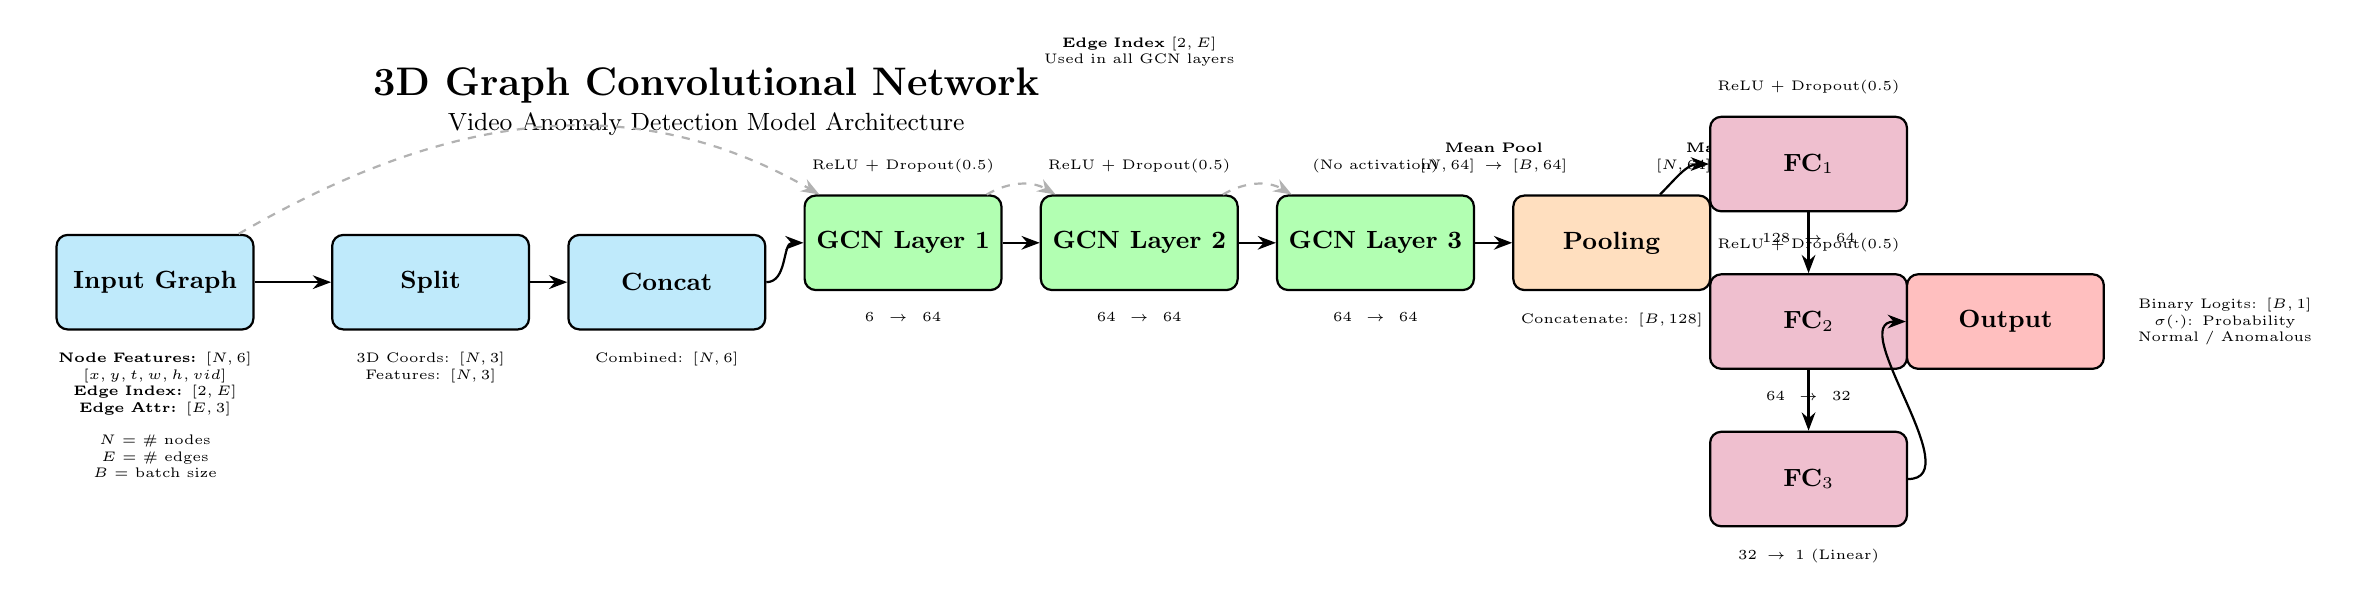
\begin{tikzpicture}[
    node distance = 1.5cm and 1.2cm,
    box/.style = {
        rectangle, 
        rounded corners=4pt, 
        minimum width=2.5cm, 
        minimum height=1.2cm, 
        text centered, 
        draw=black, 
        thick,
        font=\small
    },
    input/.style = {box, fill=cyan!25},
    gcn/.style = {box, fill=green!30},
    pool/.style = {box, fill=orange!25},
    fc/.style = {box, fill=purple!25},
    output/.style = {box, fill=red!25},
    arrow/.style = {thick, -Stealth},
    dashedarrow/.style = {thick, -Stealth, dashed, gray!60},
    dim/.style = {font=\tiny, text width=2.5cm, align=center}
]

    % Title
    \node[font=\Large\bfseries] (title) at (7,6.5) {\textbf{3D Graph Convolutional Network}};
    \node[font=\small] (subtitle) at (7,6) {Video Anomaly Detection Model Architecture};

    % === INPUT LAYER ===
    \node[input] (input) at (0,4) {\textbf{Input Graph}};
    \node[dim, below=0.15cm of input] {
        \textbf{Node Features:} $[N, 6]$\\
        $[x, y, t, w, h, vid]$\\
        \textbf{Edge Index:} $[2, E]$\\
        \textbf{Edge Attr:} $[E, 3]$
    };

    % === FEATURE PROCESSING ===
    \node[input] (split) at (3.5,4) {\textbf{Split}};
    \node[dim, below=0.15cm of split] {
        3D Coords: $[N, 3]$\\
        Features: $[N, 3]$
    };

    \node[input] (concat) at (6.5,4) {\textbf{Concat}};
    \node[dim, below=0.15cm of concat] {
        Combined: $[N, 6]$
    };

    % === GCN LAYERS ===
    \node[gcn] (gcn1) at (9.5,4.5) {\textbf{GCN Layer 1}};
    \node[dim, above=0.15cm of gcn1] {
        ReLU + Dropout(0.5)
    };
    \node[dim, below=0.15cm of gcn1] {
        $6 \to 64$
    };

    \node[gcn] (gcn2) at (12.5,4.5) {\textbf{GCN Layer 2}};
    \node[dim, above=0.15cm of gcn2] {
        ReLU + Dropout(0.5)
    };
    \node[dim, below=0.15cm of gcn2] {
        $64 \to 64$
    };

    \node[gcn] (gcn3) at (15.5,4.5) {\textbf{GCN Layer 3}};
    \node[dim, above=0.15cm of gcn3] {
        (No activation)
    };
    \node[dim, below=0.15cm of gcn3] {
        $64 \to 64$
    };

    % === GRAPH POOLING ===
    \node[pool] (pool) at (18.5,4.5) {\textbf{Pooling}};
    \node[dim, above=0.15cm of pool, xshift=-1.5cm] {
        \textbf{Mean Pool}\\
        $[N,64] \to [B,64]$
    };
    \node[dim, above=0.15cm of pool, xshift=1.5cm] {
        \textbf{Max Pool}\\
        $[N,64] \to [B,64]$
    };
    \node[dim, below=0.15cm of pool] {
        Concatenate: $[B, 128]$
    };

    % === CLASSIFIER HEAD ===
    \node[fc] (fc1) at (21,5.5) {\textbf{FC$_1$}};
    \node[dim, above=0.15cm of fc1] {
        ReLU + Dropout(0.5)
    };
    \node[dim, below=0.15cm of fc1] {
        $128 \to 64$
    };

    \node[fc] (fc2) at (21,3.5) {\textbf{FC$_2$}};
    \node[dim, above=0.15cm of fc2] {
        ReLU + Dropout(0.5)
    };
    \node[dim, below=0.15cm of fc2] {
        $64 \to 32$
    };

    \node[fc] (fc3) at (21,1.5) {\textbf{FC$_3$}};
    \node[dim, below=0.15cm of fc3] {
        $32 \to 1$ (Linear)
    };

    % === OUTPUT ===
    \node[output] (output) at (23.5,3.5) {\textbf{Output}};
    \node[dim, right=0.15cm of output] {
        Binary Logits: $[B, 1]$\\
        $\sigma(\cdot)$: Probability\\
        Normal / Anomalous
    };

    % === MAIN DATA FLOW ===
    \draw[arrow] (input) -- (split);
    \draw[arrow] (split) -- (concat);
    \draw[arrow] (concat) to[out=0, in=180] (gcn1);
    \draw[arrow] (gcn1) -- (gcn2);
    \draw[arrow] (gcn2) -- (gcn3);
    \draw[arrow] (gcn3) -- (pool);
    \draw[arrow] (pool) to[out=45, in=180] (fc1);
    \draw[arrow] (fc1) -- (fc2);
    \draw[arrow] (fc2) -- (fc3);
    \draw[arrow] (fc3) to[out=0, in=180] (output);

    % === EDGE INDEX FLOW (dashed) ===
    \draw[dashedarrow] (input) to[out=30, in=150] (gcn1);
    \draw[dashedarrow] (gcn1) to[out=30, in=150] (gcn2);
    \draw[dashedarrow] (gcn2) to[out=30, in=150] (gcn3);

    % === ANNOTATION BOXES ===
    \node[dim, above=1.5cm of gcn2, text width=4cm, align=center] {
        \textbf{Edge Index $[2, E]$}\\
        Used in all GCN layers
    };

    \node[dim, below=1.2cm of input, text width=3cm, align=center] {
        $N$ = \# nodes\\
        $E$ = \# edges\\
        $B$ = batch size
    };

\end{tikzpicture}

\end{document}
